Each report belongs to a service. Within that service, the report is identified by the \textit{sub-type} (a positive integer). Thus, a report is fully identified by a pair [x,y] where 'x' is the identifier of the service to which the report belongs (the service type, see section \ref{sec:ServConcept}) and 'y' is the identifier of the report within the service (the command sub-type).

Commands and reports within the same service have different sub-types. Thus, it is not possible for a command and a report to be identified by the same [type, sub-type] pair.  

Reports are \textit{types} which are instantiated at run-time. A report is generated by a service provider which sends it to a service user in order to provide it with information about its internal state. Thus, a report instance begins its life when the application on the service provider side (the \textit{provider application}) decides that it wishes to send some information to the application on the service user side (the \textit{user application}). 

On the service provider side, a report is configured with the information that it must carry and then it is sent to its destination (a user application). The sending of the report to the user application may be conditional on certain checks being passed. On the user side, the report performs an update action. The report encapsulates the data to be sent, the conditional checks which determine whether the report is sent, and the update action.  

The same report instance may be sent to its destination more than once. This models the situation where a service provider is issuing periodic reports to a service user. In this case, the content of the report is updated every time it is sent to its destination. 

Thus, a report is defined by its \textit{attributes}, its \textit{conditional checks} and an \textit{update action}. 

Attributes designate characteristics that are entirely defined by their value. The update actions and conditional checks designate executable functionalities that are associated to the report. The conditional checks determine whether a report is sent to its destination and the update action determines what the report does with the data it carries in its destination.

The next three subsections further define the report attributes, the report conditional checks and the report update action. The last sub-section describes the lifecycle of a report. 

%---------------------------------------------------------------------------------
\subsubsection{The Report Attributes}\label{sec:RepAttributes}

An attribute is a characteristics that is entirely defined by its value. A report has the following attributes:

\begin{itemize}
\item \textbf{Service Type}
Each report contributes to implementing a service. This attribute identifies the service that the report implements. 
\item \textbf{Report Sub-Type}
Each service is implemented by several reports. This attribute identifies the type of the report within a certain service. 
\item \textbf{Report Identifier}
A report may exist in two distinct applications (the provider application which sends the report and the user application which receives it). This attribute uniquely identifies the report instance within both applications and throughout the life of both applications.
\item \textbf{Destination}
Reports are generated by a provider application for a user application. This attribute identifies the user application for which the report is intended.
\item \textbf{Source}
Reports are generated by a provider application for a user application. This attribute identifies the provider application which issues the report.
\item \textbf{Time Stamp}
The time when the provider application makes the request to send the report to its destination.
\item \textbf{Group}
Reports sent by a provider application to the same destination are allocated to a group. This attribute identifies the group to which the report belongs. The concept of group is primarily relevant to applications which aim at PUS-compliance (see section \ref{sec:RelationshipToPUS}).  
\item \textbf{Sequence Counter}
Every time a provider application generates a report belonging to a certain source group, it increments a counter. The sequence counter attribute holds the value of this counter. The sequence counter can be used by the recipient application to check whether any reports addressed to it have been lost. 
\item \textbf{Report Parameters}
Some reports may require parameters to fully specify the actions and checks that they encapsulate. The “Report Parameters” attribute holds the value of these parameters. This attribute consists of an ordered sequence of items of primitive type. 
\item \textbf{Discriminant}
The number and type of report parameters in a report instance is not necessarily determined by the report type (i.e. different instances of the same report type may have different sets of report parameters). The discriminant is a report parameter which determines the number and type of the other report parameters. Thus, the layout of a report instance is fully determined by the triplet: [x,y,z] where 'x' is the identifier of the service to which the report belongs (the service type), 'y' is the identifier of the report within the service (the report sub-type), and 'z' is the discriminant.  The discriminant is an optional attribute. Report types which have no parameters, or which have a fixed set of parameters, have no discriminant.
\item \textbf{CRC}
A report carries a checksum which is set by the report's sender and which the recipient of the report can use to verify the integrity of the report's transmission. 

\end{itemize}


%---------------------------------------------------------------------------------
\subsubsection{The Report Conditional Checks}\label{sec:RepConditionalChecks}

A conditional check is an executable functionality which returns an enumerated value. The enumerated value reports the outcome of the check. Conditional checks are performed as part of the processing of a report in a provider application. Their outcome determines whether and when the report is sent to its destination. 

Conditional checks must have zero logical execution time. This restriction allows them to be mapped to guards in state machines. 

The following conditional checks are defined for a report on the service provider side:

\begin{itemize}
\item \textbf{Enable Check}
This check is performed when the provider application makes a request to send a report to the service user. The enable check determines whether the report instance is enabled or disabled. If the report instance is disabled, then the report is aborted. If instead the report instance is enabled, it remains in a pending state until the ready check authorizes it being sent to its destination.

\item \textbf{Ready Check}
This check is performed on a pending report instance that has passed its enable check. The ready check determines when the report instance is sent to its destination.  The report instance remains pending until the ready check is passed. When the ready check is passed, the report instance may be sent to its destination.  

\item \textbf{Repeat Check}
This check is performed on a report instance after it has been sent to its destination. The check returns either "repeat" or "no repeat". In the former case, the report instance is updated and sent again to its destination. In the latter case, it is destroyed.
\end{itemize}

On the service user side, the following conditional checks are defined for a report:

\begin{itemize}
\item \textbf{Acceptance Check}
The acceptance check is performed when the report instance is received by its destination. If the acceptance check is passed, then the report's update action is executed. If the acceptance check is not passed, then the report instance is aborted.
\end{itemize}

It should be noted that the conditional checks defined for a report on the provider side have a similar semantics as the conditional checks defined for a command on the service user side (see section \ref{sec:CmdCondChecks}). This similarity reflects the fact that out-going commands are handled in the same way as out-going reports.

%---------------------------------------------------------------------------------
\subsubsection{The Report Actions}\label{sec:RepActions}

Report actions are executable functionalities which encapsulate the actions to be performed by the command. Report actions are executed depending on the outcome of the report conditional checks. Report actions must have zero logical execution time. This restriction allows them to be mapped to actions in state machines. 

The following action is defined for a report on the service provider side:

\begin{itemize}
\item \textbf{Update Action}
Through this action, the report acquires the information which it must carry to its destination. This action is executed before the report is sent to its destination. If the report is sent more than once (i.e. if its repeat check returns "repeat" one or more times), then the Update Action is performed repeatedly every time the report must be sent to its destination.
\end{itemize} 

The following action is defined for a report on the service user side:

\begin{itemize}
\item \textbf{Update Action}
This action is executed on the user side after a report has been received by a user application and has passed its acceptance check. A report carries data to a user application. The Update Action determines what the report does with these data on the user application. 
\end{itemize} 

As in the case of the report conditional checks, it should be noted that the action defined for a report on the provider side have a similar semantics as the action defined for a command on the service user side (see section \ref{sec:CmdActions}). This similarity reflects the fact that out-going commands are handled in the same way as out-going reports.

%---------------------------------------------------------------------------------
\subsubsection{Report Lifecycle}\label{sec:RepLifecycle}

A report instance begins its life on the service provider side when the provider application creates and configures the report instance and requests it to be sent to the user application. Through the report configuration process, the provider application defines the data that the report must carry to its destination.

Nominally, on the provider side, the report can be in one single state PENDING. This corresponds to the state of a report that has passed its enable check and is waiting for its ready check to authorize the transfer of the report to the user application. 

On the user side, the report executes its acceptance check. Tyically, this check encapsulates syntactical checks which verify the integrity of the data carried by the report. If the check is passed, then the report's update action is executed. Typically, the update action might consist in updating the value of selected variables in the user application to reflect the arrival of the report, or it might consist in storing a copy of the data carried by the report into a repository. If the acceptance check is not passed, the report is simply dicarded.  

The CORDET Framework defines the logic to manage the report lifecycle but it leaves the definition of the content of the report and of its conditional checks open.

Figure \ref{fig:RepLifecycle} shows the nominal lifecycle of a report in an informal notation. In summary, the CORDET Framework pre-defines the logic to handle the transitions between the report states. It does this by defining the logic to manage the execution of the report checks and of the report actions but it leaves the definition of the content of the actions and checks open. 

The lifecycle outlined above may be repeated more than once for the same report instance. Repetition is determed by the outcome of the repeat check. The repeat check is performed at the end of the lifecycle depicted in figure \ref{fig:CmdLifecycle}. If the check returns "no repeat", then the report instance is destroyed. If instead, it returns "repeat", then the content of the report instance is updated and re-sent to its destination where it repeats the lifecycle of figure \ref{fig:RepLifecycle}.

\begin{figure}[H]
 \centering
 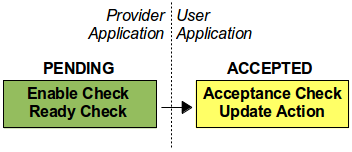
\includegraphics[scale=0.35,keepaspectratio=true]{RepLifecycle.png}
 \caption{Report Lifecycle (Informal Notation)}
 \label{fig:RepLifecycle}
\end{figure}


